
\documentclass[
	12pt
]{article}
\fontfamily{georgia}\selectfont
\usepackage[utf8]{inputenc} 
\usepackage[T1]{fontenc} 
\usepackage{mathpazo} 
\usepackage{geometry}
\usepackage{graphicx} 
\usepackage{booktabs} 

\usepackage{listings}
\usepackage{algorithm}
\usepackage{algorithmic}
\usepackage{amsmath,algpseudocode}
\usepackage{enumerate}
\usepackage[utf8]{inputenc}
\usepackage[english]{babel}
\usepackage{url}
\usepackage[utf8]{inputenc}
\usepackage[T1]{fontenc}
\usepackage{imakeidx}
\makeindex[columns=2, title=Alphabetical Index, intoc]


\title{Project  Report  \\ Software Engineering Process (SOEN 6011)\\ \vspace{20pt} ETERNITY FUNCTIONS : F3}
\author{Mileshkumar Chandulal Kotadia (ID: 40156971)\\} 
\date{August 04, 2022}

\begin{document}
\maketitle
\newpage

\tableofcontents

\newpage
\section{Introduction}
Hyperbolic functions are analogous to circular functions and trigonometric functions. It is usually possible to define hyperbolic functions by using algebraic expressions that include the exponential function (e\textsuperscript{x}) and its inverse exponential function (e\textsuperscript{-x}), where e represents Euler's constant. Here, we are going to discuss the sine hyperbolic functions, its properties, characteristics programming style and checkstyle used during development.

\section{Code Repository}
\begin{itemize}
\item URL : \url{https://github.com/mileshkotadia987/SOEN_6011_Project.git}
    \item Contributor : Mileshkumar Chandulal Kotadia (Student)
    \item Collaborator :  Abdel Rahman Idrais Alsouqi ( Teaching Assistant)
    \item Collaborator :  Somayeh Davar ( Teaching Assistant)
    \item Collaborator :  Hamed Jafarpour ( Teaching Assistant)
\end{itemize}

% problem 1
\section{Problem 1}
\subsection{Function}
\begin{itemize}
    \item Mathematically function is defined as, \textbf{sinh($x$)} =   {(e\textsuperscript{x} - e\textsuperscript{-x})}{$\div$ 2}.
\end{itemize}

\subsection{Definition}
\begin{itemize}
    \item A hyperbolic sine function is an analogy to the circular Sin function that can be found throughout trigonometry\cite{7}. When used with real numbers, it is defined by taking the area to be twice its axis, and tracing a line through the origin intersecting the unit hyperbola. This method is also used to solve ordinary differential equations of second order. \\For the given function {sinh($x$)} =   {(e\textsuperscript{x} - e\textsuperscript{-x})}{$\div$ 2} , e is the  base of natural log . Approximate value of the e is  2.71828.
\end{itemize}
\newpage
\begin{figure}[htp]
    \centering
    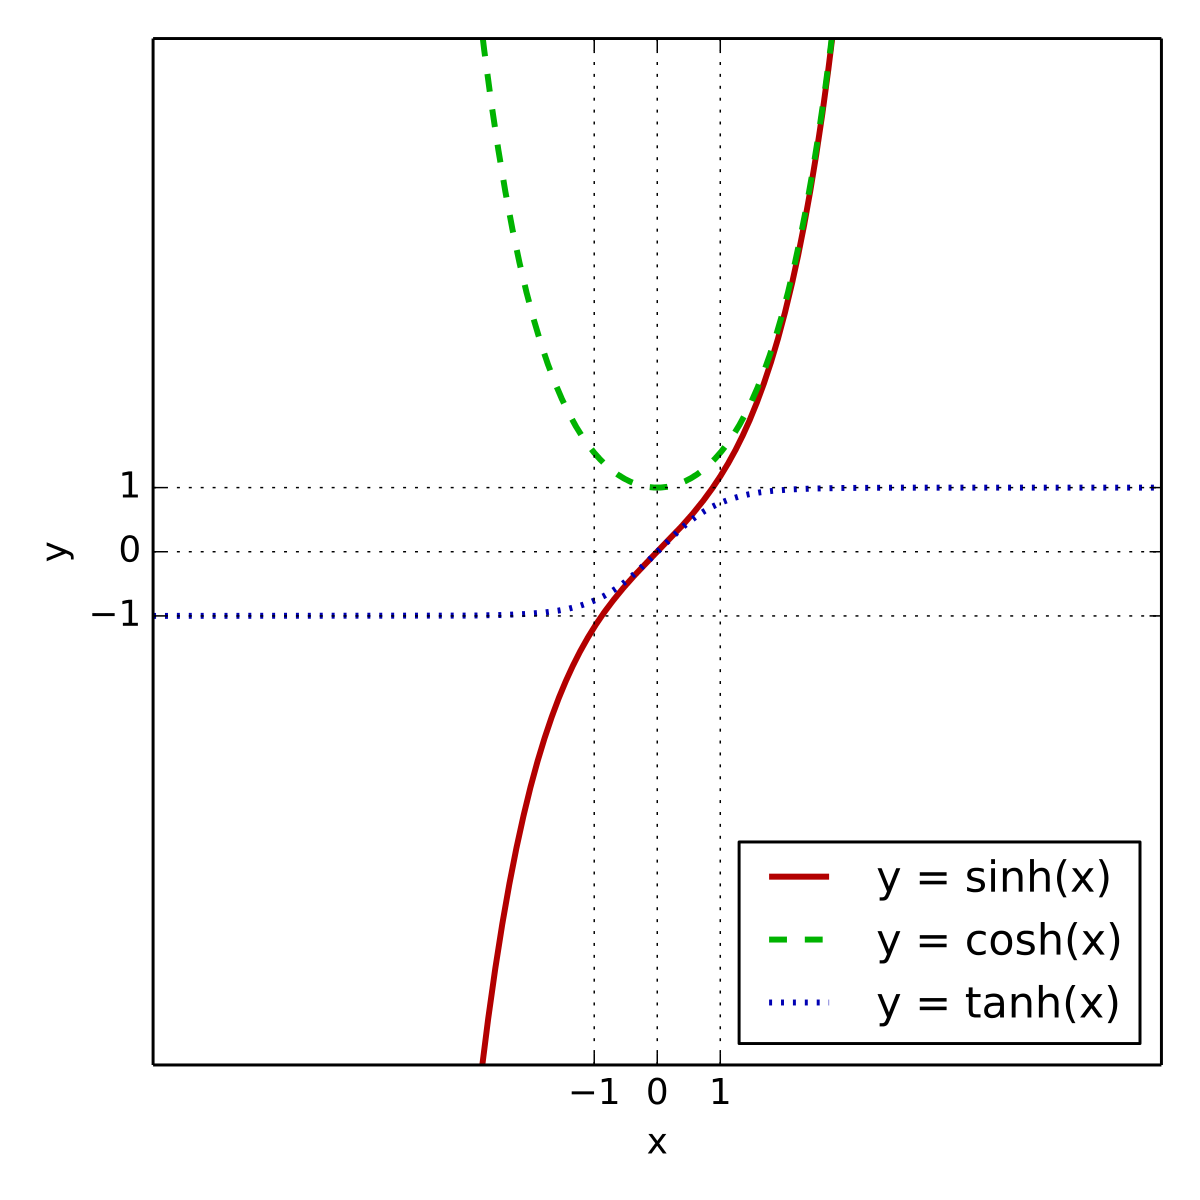
\includegraphics[width=8cm]{sin.png}
    \caption{Graph of Hyperbolic Sine Function}
    \label{sinh(x) graph}
\end{figure}

\subsection{Domain and Co-Domain}
\begin{itemize}
    \item Domain and Co-Domain of the hyperbolic sine function is  $\mathbb{R}$.
     \[ \lim_{x\to -\infty} (sinh(x)) = -\infty \] 
     \[ \lim_{x\to \infty} (sinh(x)) = \infty \]

\end{itemize}

\subsection{Characteristics}
\begin{itemize}
\item In terms of domain, the function is continuous, unbounded, and symmetric, namely odd, since sinh(-x) = -sinh(x).
\item sinh($x$) $\approx$ cosh ($x$) for large x.
\item sinh($x$) $\approx$  -cosh ($x$) for large negative x.
\item sinh($x$) has period of 2$\pi$$\imath$.
\item The graph of sinh(x) is always between the graphs e\textsuperscript{x}/2  and e\textsuperscript{-x}/2.
\end{itemize}

\subsection{Context of Use Model}
\begin{figure}[htp]
    \centering
    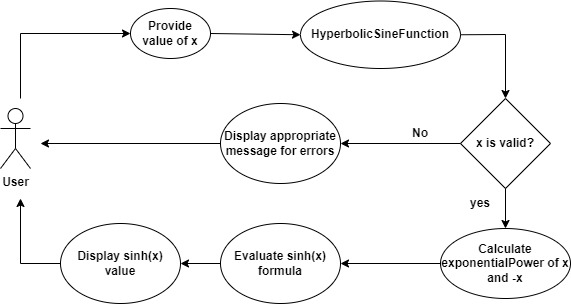
\includegraphics[width=13cm]{context.jpg}
    \caption{Context Diagram for Hyperbolic Sine Function}
    \label{sinh(x) graph}
\end{figure}

% problem 2
\section {Problem 2} 
\subsection{Functional Requirements}
\begin{enumerate}
\item\textbf{ID:} FR1\\
    \textbf{Type:} Functional\\
    \textbf{Owner:} Milesh\\
    \textbf{Dificulty:}  Easy\\
    \textbf{Description:} When the user inputs a real number x, the system should calculate and display its hyperbolic sine value.\\
    \textbf{Rationale:} To calculate $sinh(x)$
    
    \item\textbf{ID:} FR2\\
    \textbf{Type:} Functional\\
    \textbf{Owner:} Milesh\\
    \textbf{Dificulty:}  Easy\\
    \textbf{Description:} Whenever the user provides input other than a number, such as an alphabet or special character, then function should not return a value.\\
    \textbf{Rationale:} when user provides invalid input
    
\item\textbf{ID:} FR3\\
    \textbf{Type:} Functional\\
    \textbf{Owner:} Milesh\\
    \textbf{Dificulty:}  Easy\\
    \textbf{Description:} Calculated exponential value e (Euler's number)\cite{singintro1} should be in a range of finite number.\\
    \textbf{Rationale:} To calculate the exponential power of $x$.
    
\end{enumerate}

\subsection{Non-Functional Requirements}
\begin{enumerate}
\item\textbf{ID:} NFR1\\
    \textbf{Type:} Non-Functional\\
    \textbf{Owner:} Milesh\\
    \textbf{Dificulty:}  Easy\\
    \textbf{Description:} The calculator should be easy for the user to use.\\
    \textbf{Rationale:} Easiness of the application.
    
    \item\textbf{ID:} NFR2\\
    \textbf{Type:} Non-Functional\\
    \textbf{Owner:} Milesh\\
    \textbf{Dificulty:}  Easy\\
    \textbf{Description:} System should display appropriate error messages for appropriate errors.\\
    \textbf{Rationale:} The messages makes the work easier for the user.
    
\item\textbf{ID:} NFR2\\
    \textbf{Type:} Non-Functional\\
    \textbf{Owner:} Milesh\\
    \textbf{Dificulty:}  Easy\\
    \textbf{Description:} The calculator should provide accurate and precise answer.\\
    \textbf{Rationale:} It helps the user to solve complex mathematical problems.
\end{enumerate}

\subsection{Assumptions}
\begin{enumerate}
    \item 
    Assumption-1 \newline Description: The domain of a hyperbolic sine function can be expressed mathematically as a set of all possible real numbers. In order to implement the function on the computer, Java will be used as a programming language, so there are limitations on user input. The range of user input should be in between - 1.79769313486231570E+308 to + 1.79769313486231570E+308.

    \item
    Assumption-2 \newline Description: Due to the type of data used, there is a limit on the number of decimal points considered for the calculation if decimal numbers are input. The first 10 decimal points will be considered a significant decimal point.

    \item
    Assumption-3 \newline Description: Mathematically value of e is calculated as\newline
    e = 1/0! + 1/1! + 1/2! + 1/3! + ... = 2.7182818284590452353602875.... , Since there is a limitation of datatype in java programming language, the infinite calculation is not possible\cite{hyperbolicfunctions}. Therefore, implementing the calculation of e will provide the value of e = 2.7182815255731922.
    \item
     Assumption-4 \newline Description: Because programming languages have restrictions on data types, there are also restrictions on output value. Output value cannot exceed what the datatype permits. The output will be constrained and less than the maximum permissible value of 1.79769313486231570E+308 and greater than the lowest allowed value even if the user enters the maximum allowed value (maximum that data type may carry) -1.79769313486231570E+308\cite{range}.
\end{enumerate}

% Problem 3
\section{Problem 3}
\subsection{Algorithm 1}\newline
\textbf{Description:}
For a given value of x, Algorithm 1 determines the hyperbolic sine function's value. There is no explicit calculation of the value of e in this algorithm. The below mentioned function EXPONENTIALPOWER() uses the Taylor series to determine the value of e power x \cite{sinhintro}.\newline 
We cannot calculate Taylor series that proceed indefinitely since the algorithm must end at some point. Due to this,  the counter value is 10, which also meet above mentioned Assumption 3 and allows the algorithm to end with the highest precision possible up to 10 decimal places.\newline After computing the value of $e\textsuperscript{x}$ and $e\textsuperscript{-x}$ , value for the hyperbolic sine function is calculated.\\
\newpage
\newline\textbf{Advantage:}
\begin{itemize}
    \item There is no recursion used in the algorithm which means that the execution stack will need less space.
    \item Calculation does not need any explicit function call. $e$
\end{itemize}
\textbf{Disadvantage:}
\begin{itemize}
    \item The maximum accuracy of output is 10 decimal places.
\end{itemize}
\textbf{Reason to select  algorithm:}
\begin{itemize}
    \item No Recursion and Taylor Series Efficiency.
\end{itemize}
\textbf{Mind Map:}
     \begin{figure}[htp]
    \centering
    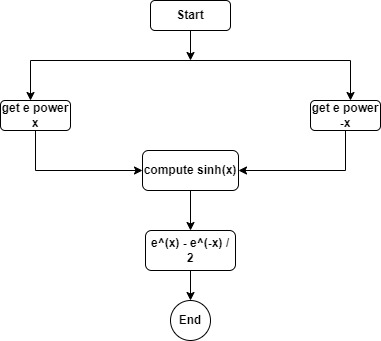
\includegraphics[width=10cm]{m1.jpg}
    \caption{ Mind Map of Algorithm 1}
    \label{Project Modules}
\end{figure}
\newpage
\textbf{Pseudocode Algorithm 1:}
\begin{algorithm}
\caption{Calculate sinh($x$) =   {($e\textsuperscript{x} - e\textsuperscript{-x}$)}{$\div$ 2}}
\begin{algorithmic} 
\REQUIRE $x \neq null$
\STATE $e\textsuperscript{x} \leftarrow $EXPONENTIALPOWER($x$)
\STATE $e\textsuperscript{-x} \leftarrow $EXPONENTIALPOWER($-x$)
\STATE $ sinhx \leftarrow (e\textsuperscript{x} - e\textsuperscript{-x})\div 2 $
\Statex
\Function{ExponentialPower}{$x$} 
  \STATE $exponent \leftarrow x$
  \STATE $fractional \leftarrow exponent$
  \STATE $result \leftarrow 1+exponent$
  \STATE $counter \leftarrow 1$

\WHILE{$partial \neq result$}
     \STATE $counter \leftarrow $counter$+1$\\
    \STATE $fractional* \leftarrow exponent/counter$
    \STATE $partial \leftarrow result$
    \STATE $result+ \leftarrow fractional$
    
\ENDWHILE
\State \Return $result$
\EndFunction
\end{algorithmic}
\end{algorithm}\\


\subsection{Algorithm 2} \newline\newline
\textbf{Description:}
\newline\normalfont Algorithm 2 also determines the hyperbolic sine function's value.
This algorithm directly calculates the value of $e$. With the use of the EXPPOWER function, the method utilises the value of e for computing $e\textsuperscript{x}$ and $e\textsuperscript{-x}$.
Since the algorithm must end at some point, the algorithm's counter value of 10 causes it to end with the greatest precision possible up to 10 decimal places. Hence, it helps in satisfying the above mentioned Assumption 3.
Algorithm uses a Recursion functionality to calculate $e\textsuperscript{x}$ and $e\textsuperscript{-x}$.\newline
\newline\textbf{Advantage:}
\begin{itemize}
    \item Modularization becomes easy.
    \item The computation of e does not take $x$ into account like Algorithm 1, making it simple to improve the approximation of value $e$ as needed.
\end{itemize}
\newline\textbf{Disadvantage:}
\begin{itemize}
    \item Recursion is used to calculate exponential power, which takes up more execution space on the stack.
    \item To compute $e$, an explicit function call is needed.
\end{itemize}
\newline\textbf{Reason to select  algorithm:}
\begin{itemize}
    \item adaptability in obtaining a greater approximation of $e$. This aids in getting precise results for sinh ($x$).
\end{itemize}
\textbf{Mind Map:}
     \begin{figure}[htp]
    \centering
    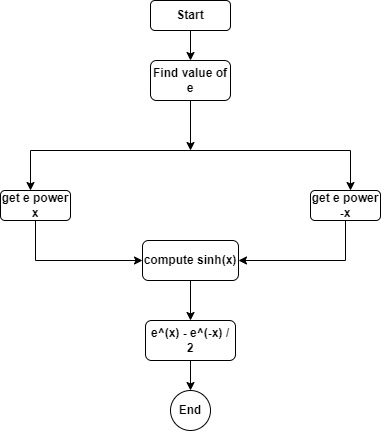
\includegraphics[width=9cm]{m2.jpg}
    \caption{ Mind Map of Algorithm 2}
    \label{Project Modules}
\end{figure}
\newpage
\noindent\textbf{Pseudocode Algorithm 2:}
\begin{algorithm}
\caption{Calculate sinh($x$) =   {($e\textsuperscript{x} - e\textsuperscript{-x}$)}{$\div$ 2}}
\begin{algorithmic} 
\REQUIRE $x \neq null$
\STATE $ sinhx \leftarrow (e\textsuperscript{x} - e\textsuperscript{-x})\div 2 $
\STATE $e \leftarrow $FINDE()
\STATE $e\textsuperscript{x} \leftarrow $EXPPOWER($e$,$x$)
\STATE $e\textsuperscript{-x} \leftarrow $EXPPOWER($e$,$-x$)
\newline
\Function{FINDE()}{}
   \STATE $e \leftarrow 1$
\STATE $decimalCount \leftarrow 10$ 
\WHILE{$decimalCount \textgreater 0$}
     $e = 1 + ($e$) $\div$ $decimalCount;\newline
     \STATE $decimalCount \leftarrow $decimalCount$-1$
\ENDWHILE
    \State \Return $e$
\EndFunction
\newline
\Function{EXPPOWER}{$e$,$x$}
\IF{$x = 0$}
\State \Return $1$
\ENDIF
\IF{$x \% 2 == 0$}
    \State \Return $EXPPOWER(e,x\div 2) * EXPPOWER(e,x\div 2)$
\ELSE
\State \Return $x * EXPPOWER(e,x\div 2) * EXPPOWER(e,x\div 2) $
\ENDIF
\EndFunction
\end{algorithmic}
\end{algorithm}

%problem 4
\section{Problem 4}
\subsection{Programming style}
Style guides provide uniformity and predictability throughout your project\cite{styleguide}.
We as a team had decided to use Google Programming style for java. 
Reasons to use Google Style guide :
\begin{itemize}
    \item It makes reading code simpler.
    \item It improves predictability of file and variable names.
    \item Because of this, programmers may concentrate on logic rather than stylistic decisions.
    \item Using shortcuts, programmers may reformat code by importing the style guide into their IDE\cite{googlestyleguide}.
\end{itemize}
\subsection{Debugger}
When programming, a debugger aids in examining erratic behaviour.
I used the Intellij IDE and Intellij Debugger to implement the sinh($x$) function using Java.\\
\newline\textbf{Advantages of Intellij Debugger}
\begin{itemize}
    \item Analyze the use of memory
    \item support for remote Java application debugging
    \item assistance with conditional break points (stop debugger only when some condition occur)\cite{debuggingtools}.
    \item Set up and customise breakpoints and watchpoints.
    \item Evaluate expressions
    \item Debugging sessions are interrupted and resumed

\end{itemize}
\begin{figure}[htp]
    \centering
    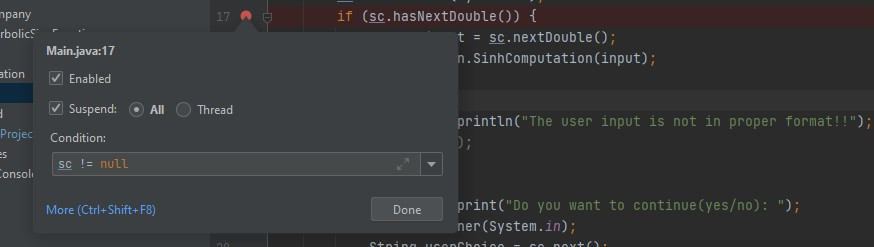
\includegraphics[width=12cm]{inlineDebug.jpg}
    \caption{Support for conditional break points}
    \label{Support for conditional break points}
\end{figure}
\newpage
\textbf{Disadvantage of Intellij Debugger}
\begin{itemize}
    \item It is not feasible to use Intellij Debugger alone; it is a component of the Intellij IDE for Java.
    \item When compared to Eclipse IDE, Intelij takes greater system RAM to function\cite{eclipsevsintelij}. High-end setups are required for the InteliJ debugger.
\end{itemize}

\subsection{Quality Attributes}
\begin{enumerate}
    \item \textbf{Correctness}
    \begin{itemize}
        \item Using Junit test cases, the accuracy of the implemented software is confirmed.
        \item In test
cases, the expected result is calculated from\newline
\url{https://keisan.casio.com/exec/system/1223039747}, it is leading calculator manufacturing
company \cite{casio}. \
\item The computed value from the implemented function is compared to the expected value that was obtained and is asserted.
    \end{itemize}
    \begin{figure}[htp]
    \centering
    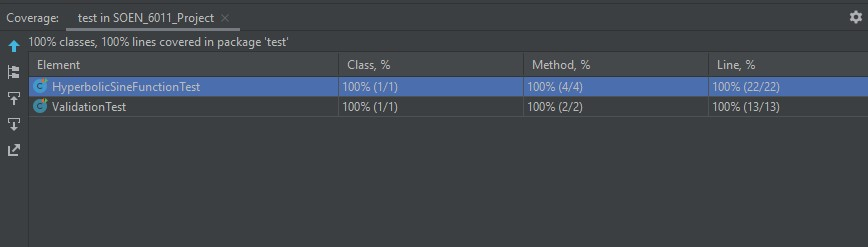
\includegraphics[width=12cm]{codecoverage.jpg}
    \caption{Code coverage for the Project}
    \label{Code coverage for the Project}
\end{figure}
\item \textbf{Efficiency}
\begin{itemize}
    \item No nested loops are used during implementation.
    \item There is no recursion in the implementation.
    \item JIt takes 74 ms (0.074 seconds) to complete a unit test suit (5 test cases) that runs all implemented functions.
     \begin{figure}[htp]
    \centering
    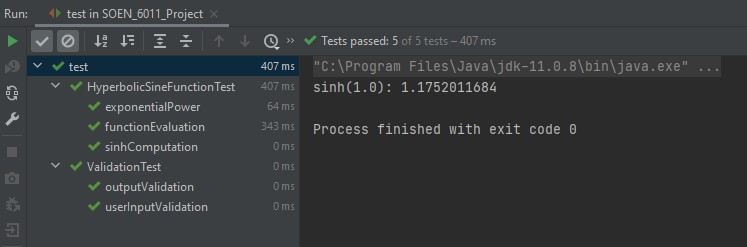
\includegraphics[width=12cm]{testcases.jpg}
    \caption{ Junit test suit Execution time for all functions}
    \label{Execution time for all functions}
\end{figure}
\end{itemize}\newpage
\item \textbf{Maintainable}
\begin{itemize}
    \item Modular architecture helps to ensure maintainability.
For sine function computation and function validation, there is a separate class. For instance, all that has to be changed is the validation class if we wish to alter the criteria for validating user inputs and output.
\item Comments are added with the proper details.
\end{itemize}
 \begin{figure}[htp]
    \centering
    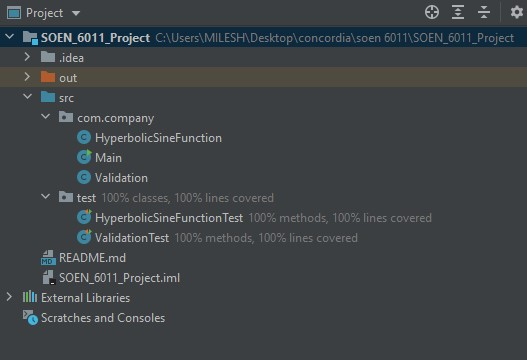
\includegraphics[width=12cm]{module.jpg}
    \caption{ Project Modules}
    \label{Project Modules}
\end{figure}
\item \textbf{Robust}\\
Robustness is achieved by ,
\begin{itemize}
    \item Strict validation is performed on user input to ensure that only numeric values are entered.
    \item Prior to computation, the input is verified to ensure that the data type is supported.
    \item Verifying the output range, and displaying the appropriate error message to the user if the output exceeds what the data type can handle.\\
\end{itemize}
\item \textbf{Usability}
\newline Usability is achieved with the help of,
\begin{itemize}
    \item Providing a straightforward, user-friendly text UI.
    \item Displaying appropriate error messages as needed.
    \item Displaying appropriate directions for following up on the outcome.(Figure \ref{Screenshot of  UI})
    \item Any system having a JVM may run an exported application as an executable jar file.
\end{itemize}
\begin{figure}[htp]
    \centering
    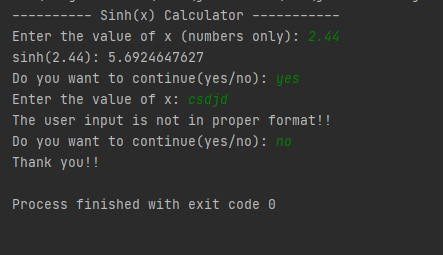
\includegraphics[width=12cm]{ui.jpg}
        \caption{Screenshot of  UI}
    \label{Screenshot of  UI}
\end{figure}
\end{enumerate}
\newpage
\subsection{CheckStyle}
Programmers can use Checkstyle as a development tool to build Java code that follows a coding standard\cite{checkstyle}. The sinh($x$) function is implemented using Google Checkstyle. \\ \\
\textbf{Advantage}
\begin{itemize}
    \item Simple to set up for continuous integration. You may impose it on the project build process such that it fails if there is a checkstyle warning or error.
    \item Checkstyle makes code understandable by checking for layout and formatting errors.
\end{itemize}
\textbf{Disadvantage}
\begin{itemize}
    \item There is no check that identifies superfluous type casts.
    \item No search for inactive public methods is performed.
\end{itemize}

%problem 5
\section{Problem 5}
\subsection{Junit standards}
 One may better comprehend and appreciate the entire benefit of testing in software development with the aid of improved presentation and structure of the use of JUnit and testing. The Junit procedures listed in are applied wherever practical.
\subsection{Traceability to Requirements}
\begin{enumerate}
    \item \textbf{Requirement 1}\\
    Junit test case(s) : userInputValidation() , functionEvaluation() \\
    Description : These tests confirm that if the user enters a legitimate numeric value, the function will display the correct, accurate computed value.
    \item
    \textbf{Requirement 2} \\
    Junit test case : userInputValidation() \\
    Description : This test determines if the function displays the appropriate error message when the user enters an erroneous value (alphabet or special characters).
    \item
   \textbf{Requirement 3} \newline
    Junit test case : exponentialPower() \\
    Description : This test determines if the computed value of e (Euler's number) is finite or not.
\end{enumerate}
\subsection{Traceability to Assumptions}
\begin{enumerate}
    \item \textbf{Assumption 1}\\
    Junit test case(s) : userInputValidation(). \\
    Description : when user inputs valid number value but more than what datatype can handle then function should show  proper error message.This scenario is verified by given tests.
    \item \textbf{Assumption 2}\\
    Junit test case(s) : sinhComputation(). \\
    Description : When a user enters a legitimate value but there are more than 10 decimal places, the function should only consider the first 10 places as meaningful decimal places.
    \item
    \textbf{Assumption 3} \\
    Junit test case(s) : exponentialPower(). \\
    Description : By using the epowerx(double $x$) function and supplying x as 1, this test validates the value of e.
    \item
   \textbf{Assumption 4} \\
    Junit test case(s) : outputValidation(). \\
    Description : The function should return false if the user inputs a valid numeric number and the value is within the datatype's permitted range but the output is more or less than what the datatype can hold.
\end{enumerate}

\printindex
\nocite{*}
\bibliographystyle{unsrt}
\bibliography{ref}
\end{document}
